\section{Geometric Insights}
\label{sec:analytic}
Before launching into the computational analysis, some useful insight can be gained regarding the winning regions through geometric constructions.  

The visualizations produced in this manner 

In this section, we will derive analytical characterizations for the winning sets for the defender ($F_D$ and $R_D$) during each individual stage of the game. The union of these sets constitutes an under-approximation of the total winning set $W_D$ and provide insights to the numerical computation of $W_D$ as will be discussed in Sec~\ref{sec:hj_formulation}.

We represent the 4D set $F_D$ as a union of slices $F_D(x^a)$ parameterized by the initial location of the attacker $x^a\in D$, where each slice $F_D(x^a)$, defined by
\begin{align*}
F_D(x^a) \triangleq \{x^d\in D^-: (x^a,x^d) \in F_D\},
\end{align*}
is a 2D set containing the initial locations starting from which the defender can always stop the attacker from capturing the flag whenever the attacker's initial location is $x^a$. The set $R_D$ is decomposed similarly as $R_D =\cup_{x^a\in D} R_D(x^a)$ with 
\begin{align*}
R_D(x^a) \triangleq \{x^d\in D^-: (x^a,x^d) \in R_D\}.
\end{align*}

To simplify the discussion, we shall mainly focus on an extreme case, where the radius of the capture region is $r_c =0$. In this case, the attacker is tagged only when the two players are at exactly the same location. Denote the stop return and stop flag sets in this extreme case as $R_D^0(x^a)$ and $F_D^0(x^a)$, respectively. The approach can be easily extended to handle the case with $r_c>0$.
In the rest of this section, unless otherwise stated, we always assume that $r_c=0$. 

\subsection{Characterization of $R_D^0(x^a)$}
\label{sec:RD0}

Consider the case when the attacker is attempting to arrive at the return region $R$, perhaps after capturing the flag, as shown in Figure~\ref{fig:RD0}.  It is clear that the attacker will be unable to safely return if it is horizontally aligned with the defender, that is, if the defender is located along the line $c_2 - c_5$.  since the defender can prevent the attacker from reaching $R$ by simply paralleling    

This subsection focuses on the second stage of the game, where the attacker is located at some generic position $x^a\in D$ at time $t=0$ and its only goal is to reach the return region. On the other hand, the defender tries to stop the attacker getting back to the return region. 

The attacker is called {\em return-blocked} by the defender at time $t\ge 0$ if 
\begin{align*}
x^d_1(t)<x_1^a(t) \text{ and } x^d_2(t) = x^a_2(t).
\end{align*}
Clearly, whenever the attacker is return-blocked, the defender wins this part of the game by using the following control
\begin{align*}
d_2(t) = \dot x^a_2(t)=u_2(t) \text{ and } d_1(t) = \sqrt{v_{\max} - d_2(t)^2}. 
\end{align*}
Under this control input, the defender stays vertically aligned with the attacker and uses the remaining control effort to approach the attacker horizontally. Therefore, the attacker can not get into the return region without being captured. 

With the above scenario in mind, the characterization of the set $R_D^0(x^d)$ can be easily obtained as illustrated in Fig.~\ref{fig:RD0}. Let $o$ and $c_3$ be the two left corners of the game domain $D$. Let $c_2=x^a$ be point corresponding to $x^a$ in the figure. Draw a circle around the center $o$ with radius $\|o-c_2\|$ and let $c_1$ be the intersection point of this circle with the left boundary of $D$. Let $S_1$ be the circular sector enclosed by the two radii $oc_1$ and $oc_2$. Similarly, draw another circle centered around $c_3$ with radius $\|c_3-c_2\|$, which intersects the left boundary of $D$ at $c_4$. Denote $S_2$ the circular sector enclosed by the two raddi $c_3c_2$ and $c_3c_4$. We claim that the stop return set with $r_c = 0$ is just the intersection of the two sectors $S_1$ and $S_2$, i.e.,
\begin{align}
\label{eq:RD0}
R_D^0(x^a) = S_1\cap S_2.
\end{align} 

To show this claim, we shall verify the following two statements: (i) if the defender starts inside the intersection, then there exists a defending strategy that can keep the attacker away from the return region for any finite time, no matter what the attacker does; (ii) if the defender starts outside the intersection, there exists an attacking strategy that guarantees a safe return for the attacker no matter what the defender does. 

\begin{figure}[htbp]
	\centering
	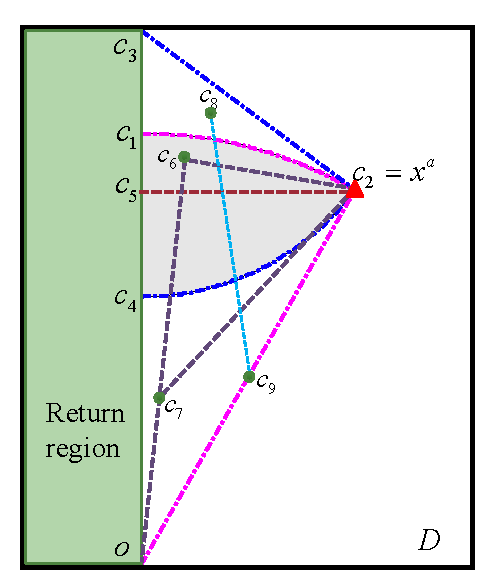
\includegraphics[width=0.7\columnwidth]{figures/RD0}
	\caption{\textbf{Illustration for deriving the stop return set $R_D^0(x^a)$}}
	\label{fig:RD0}
\end{figure}

We first assume that the initial defender location $x^d\in S_1\cap S_2$ and denote its corresponding point in Fig.~\ref{fig:RD0} by $c_6$. Without loss of generality, we assume that $c_6$ is above the line $c_5c_2$. In this case, we propose that the defender travels at its maximum speed towards point $o$ along the line $c_6o$. As mentioned before, the defender wins this part of the game whenever the attacker becomes return-blocked. The only way for the attacker to avoid being blocked is to cross the line $c_6o$ at some point $c_7$ before the defender reaches that point. Since the two players have the same maximum speed, this can happen only if $\|c_2-c_7\|\le\|c_6-c_7\|$, which is clearly impossible. The case when $c_6$ is below the line $c_5c_2$ can be argued similarly by letting the defender travel at the maximum speed towards point $c_3$ along the line $c_6c_3$. Since the defender knows whether it is above or below $c_5c_2$ at any time, it can always win the game if it starts inside $S_1\cap S_2$. 

We now assume that $x^d\notin S_1\cap S_2$ and $x^d_2>x^a_2$ (above line $c_5c_2$). In this case, if the attacker moves at its maximum speed along line $c_2o$, then the defender can not capture the attacker because for any point $c_9$ on the line $c_2o$, $\|c_8-c_9\|\ge \|c_2-c_9\|$. The case where $x^d_2<x^a_2$ can be argued similarly. 

According to the above discussion, the set $R_D^0(x^a)$ is indeed given by the intersection of the two sectors $S_1$ and $S_2$, and thus can be immediately computed once $x^a$ is known. 

\subsection{Characterization of $F_D^0(x^a)$}
\label{sec:FD0}
We now focus on the first stage of the game where the only goal of the attacker is to get the flag, namely, enter the flag region, while the defender tries to stop the attacker from achieving this goal without considering the second stage of the game at all. The winning zone of the defender for this decoupled part of the game is the stop flag set $F_D^0(x^a)$ (assuming $r_c=0$) and can be characterized in a similar manner as done for the stop return set in the last subsection. 

The attacker is called {\em flag-blocked} if it is radially aligned with the defender with respect to the circular flag region $F$ and is farther away from $F$ than the defender. Clearly, whenever the attacker is flag-blocked, the defender can always stop it from getting the flag by traveling at the same angular velocity as the attacker and using the remaining control effort to approach the attacker radially. Therefore, it suffices to characterize the set of initial defender locations that can always result in a flag-block situation no matter what the attacker does. 

\begin{figure}[tbp]
	\centering
	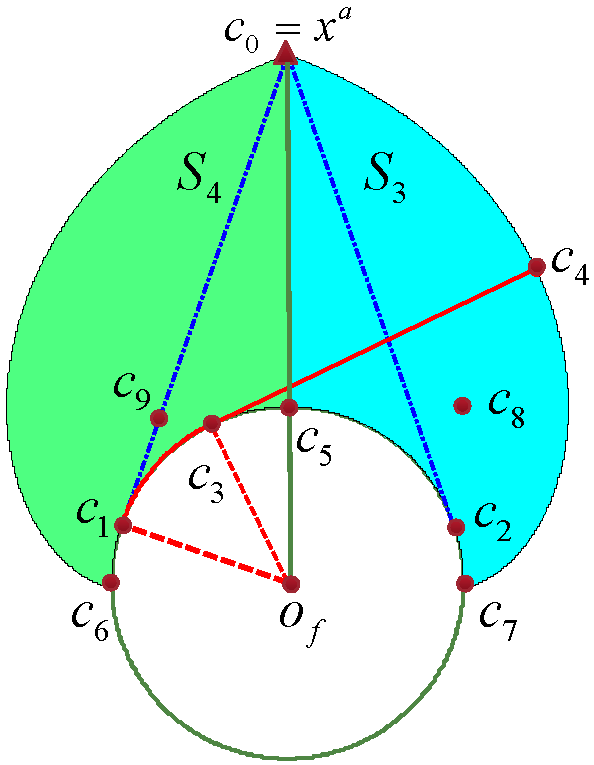
\includegraphics[width=0.65\columnwidth]{figures/FD0}
	\caption{\textbf{Illustration of the stop flag set $F_D^0(x^a)$}}
	\label{fig:FD0}
\end{figure}
Following the above idea, the derivation of $F_D^0(x^a)$ is illustrated in Fig.~\ref{fig:FD0}, where $o_f$ is the center of the flag region, $c_o$ is the point corresponding to $x^a$, $c_1$ and $c_2$ are the two points for which the two line segments $c_oc_1$ and $c_oc_2$ are tangent to the circular flag region $F$, and $c_5$ is the point where the line segment $c_oo_f$ intersects the $F$. For any point $c_3$ on the circle, denote by $arc(c_3,c_1)$ the circular arc segment between $c_1$ and $c_3$, and by $\|arc(c_3,c_1)\|$ the length of the arc segment. When $c_3$ is sufficiently close to $c_1$, there always exist another point $c_4$ satisfying
\begin{align*}
\|c_4 - c_3\|+\|arc(c_3,c_1)\| = \|c_1-c_o\|. 
\end{align*}
As $c_3$ moves away from $c_1$ clockwise along the circle, the corresponding point $c_4$ changes gradually from $c_o$ to a point on the circle $c_7$. Let $S_3$ be the set enclosed by the curve segment from $c_o$ to $c_7$, the circular segment $arc(c_7,c_5)$ and the line segment $c_5c_o$. Let $S_4$ be the reflection image of $S_3$ with respect to the line $c_oo_f$. A key property of the set $S_3$ (resp. $S_4$) is that for any point $c_8$ in the set and any point $c_9$ on the line segment $c_oc_1$ (resp. $c_oc_2$), the length of the shortest path, connecting the two points $c_8$ and $c_9$ without passing through the interior of the flag circle, is less than $\|c_9-c_o\|$. According to this property, if the defender starts inside $S_3$ (resp. $S_4$) and travels at the maximum speed along the shortesft feasible path\footnote{For example, the shortest feasible path from $c_4$ to $c_1$ is the line segment $c_4c_3$ followed by the circular arc from $c_3$ to $c_1$ as shown in Fig.~\ref{fig:FD0}} to $c_1$ (resp. $c_2$), it can always flag-block the attacker. On the other hand, if the defender's initial position is outside $S_3\cup S_4$ and to the right (resp. left) of the line $c_oo_f$, the attacker can always reach the flag region by traveling at its maximum speed towards $c_1$ (resp. $c_2$) along the line $c_oc_1$ (resp. $c_oc_2$) without being blocked or captured. Therefore, following a similar argument as the one used to justify~(\ref{eq:RD0}), we can conclude that
\begin{align}
F_D^0(x^a) = S_3 \cup S_4. 
\end{align}

\subsection{Applications and Limitations}
We now briefly describe how our analytical results can be used to guide the decision making for the defender. As discussed in the last two subsections, the sets $R_D^0(x^a)$ and $F_D^0(x^a)$ can be easily determined once the location of the attacker $x^a$ is given.

At any time $t>0$ during the game, the defender knows the attacker location $x^a(t)$ and whether it has already captured the flag or not. If the attacker already has the flag, then the defender should check whether its location $x^d(t)\in R_D^0(x^a(t))$ or not. If $x^d(t)\in R_D^0(x^a(t))$, then the defender is guaranteed to win the game by following the winning defending strategy described in Section~\ref{sec:RD0}. However, if $x^d(t)\notin R_D^0(x^a(t))$, then the defender may lose the game if the attacker plays optimally. 

On the other hand, if at time $t$ the attacker has not captured the flag, then the defender needs to check whether its location $x^d(t)\in R_D^0(x^a(t))\cup F_D^0(x^a(t))$ or not. If $x^d(t)\in F_D^0(x^a(t))$, then the attacker can stop the attacker from getting the flag by following the defending strategy described in Section~\ref{sec:FD0}. If $x^d(t)\in R_D^0(x^a(t))\setminus F_D^0(x^a(t))$, then the defender may lose the first stage of the game but is guaranteed to block the return of the attacker by following the defending strategy in Section~\ref{sec:RD0}. In other words, in this case, the defender needs to give up the first stage of the game in order to guarantee the winning of the second stage of the game and in turn the whole game. 

The case where our analytical results does not offer an exact answer to the solution of the game is when the attacker has not captured the flag and $x^d(t)\notin R_D^0(x^a(t))\cup F_D^0(x^a(t))$. In this case, the defender can not win the first stage of the game. In addition, since $x^d(t)\notin F_D^0(x^a(t))$, the attacker can achieve a safe return if it does not attempt to capture the flag. However, the goal of capturing the flag may not be consistent with the goal of achieving a safe return. Therefore, the defender may have an opportunity to win the overall game. Unfortunately, the set of initial locations that guarantee the winning for the defender can not be characterized analytically in this case.